% arara: xelatex

\documentclass[11pt]{article}
\synctex=1

\usepackage{listings}
\usepackage{graphicx}
\usepackage{multicol}
\setlength{\columnsep}{12.5pt}
\usepackage{caption}
\usepackage{floatrow}
\usepackage{cprotect}
\usepackage{enumitem}

\usepackage{calc}
\usepackage{array,booktabs}
\usepackage[usenames,dvipsnames,table]{xcolor}
\usepackage{tikz}
\usetikzlibrary{calc}
\pgfdeclarelayer{background}
\pgfdeclarelayer{foreground}
\pgfsetlayers{background,main,foreground}

% Macro para el listado con los atajos de teclado
\NewDocumentEnvironment{keys}{mmm}
{
\phantom{\hspace{-1.425\baselineskip}}
\begin{tikzpicture}
\rowcolors{1}{}{#3}
	\node (tbl) [inner sep=0pt] \bgroup
	\begin{tabular}{p{0.55\textwidth}p{0.4\textwidth}}
	\rowcolor{#2}
	\multicolumn{2}{l}{\normalsize\textbf{\color{white}{#1}}}
	\parbox{0pt}{\rule{0pt}{0.3ex+\baselineskip}}\\
}
{
	\arrayrulecolor{#2}\specialrule{.17em}{0em}{.2em}
	\end{tabular}\egroup ;
\end{tikzpicture}
}

% Márgenes y espaciado
\usepackage[
	a4paper, % Tamaño del papel
	top=2.5cm, % Márgen superior
	bottom=2cm, % Márgen inferior
	left=2.25cm, % Márgen izquierdo
	right=2.25cm, % Márgen derecho
	footskip=1cm, % Space from the bottom margin to the baseline of the footer
	headsep=0.5cm, % Space from the top margin to the baseline of the header
	headheight=1cm, % Height of the header
	%showframe
]{geometry}

\usepackage{fontspec} % Required for specifying custom fonts under XeLaTeX

\setmainfont[
Path = /usr/share/fonts/TTF/,
ItalicFont = DejaVuSerif-Italic.ttf,
BoldFont = RobotoCondensed-Bold.ttf,
BoldItalicFont = RobotoCondensed-BoldItalic.ttf
]{DejaVuMathTeXGyre.ttf}

\setmonofont{Iosevka Fixed SS05}

\usepackage[spanish]{babel} % Idioma del documento: Español

\usepackage[nobottomtitles*]{titlesec}
\titlespacing*{\section}{0pt}{7.5pt}{8pt} % Spacing around section titles, the order is: left, before and after

% Colores
\usepackage{xcolor}
\definecolor{mycolor}{HTML}{3CB5D6}

% Encabezado y pie de página
\usepackage{fancyhdr}
\pagestyle{fancy}
\fancyhf{}
\lhead{\leftmark}
\rhead{{\bfseries\thepage}}
\renewcommand{\headrulewidth}{2pt}
\renewcommand{\footrulewidth}{0pt}

% Notas de colores
\usepackage{tcolorbox}
\tcbuselibrary{skins}
\newtcolorbox{mybox}[1]{
width=\textwidth,
colback=mycolor!10,
colbacktitle=mycolor,
boxrule=-0.1pt,
center,
fonttitle=\bfseries,
title={\hspace*{-8pt}#1}, % Sin indentación en el título
sharp corners
}

% Enlaces clicables
\usepackage[colorlinks=true, linkcolor=mycolor, urlcolor=mycolor]{hyperref}

\begin{document}

\pagestyle{empty}
\vspace*{.3\textheight}
{\hfill\Huge\itshape\textcolor{mycolor}{\textbf{Artix Linux}}\par}

{\hfill\Large Guía de Usuario\par}

\clearpage

\section{Introducción}

Este documento pretende ser una guía para que termines de configurar tu instalación de Artix Linux. Hay cosas que no son razonables/posibles auto-configurar y esta guía contiene instrucciones sobre como configurar servicios como cronie, libvirt, etc.

\vspace{10pt}

\noindent También contiene instrucciones sobre como usar el entorno de trabajo del instalador.

\begin{mybox}{Nota}
Cualquier texto que veas coloreado en azul es un hiper-vínculo y si le haces doble clic, este te llevará a la página web a la que hace referencia o que explica de que se esta hablando.
\end{mybox}

\section{Atajos de teclado}

\href{https://dwm.suckless.org}{Dwm} es el programa que se encarga de repartir el espacio en pantalla entre nuestras ventanas \textit{(aplicaciones gráficas)}. Hay una cantidad enorme de \href{https://www.youtube.com/results?search_query=dynamic+window+manager}{videos sobre dwm}, como funciona y sus ventajas. Aquí veremos simplemente los atajos de teclado configurados:

\vspace{10pt}

\begin{keys}{Atajos de teclado}{mycolor}{mycolor!15}
Abrir este documento & \texttt{Alt Izq. + Ctrl + H} \\
Abrir lanzador de comandos & \texttt{Alt Izq. + P} \\
Abrir lanzador de aplicaciones & \texttt{Alt Izq. + Shift + P} \\
Abrir dmenu (calculadora) & \texttt{Ctrl + Alt Izq. + P} \\
Abrir dmenu (contraseñas) & \texttt{Ctrl + P} \\
Abrir terminal & \texttt{Alt Izq. + Shift + Intro} \\
Aumentar el espacio entre ventanas & \texttt{Alt Izq. + Ctrl + ,} \\
Disminuir el espacio entre ventanas & \texttt{Alt Izq. + Ctrl + .} \\
Configurar pantallas & \texttt{Alt Izq. + F1 / Alt + Shift + F1} \\
Abrir Navegador \textit{(Firefox)} & \texttt{Alt Izq. + F2} \\
Abrir Explorador de archivos & \texttt{Alt Izq. + F3} \\
Explorador de Archivos (/run/media)& \texttt{Alt Izq. + Shift + F3} \\
Abrir el reproductor de música & \texttt{Alt Izq. + F4} \\
Montar dipositivo Android & \texttt{Alt Izq. + F5} \\
Desmontar dipositivo Android & \texttt{Alt Izq. + Shift + F5} \\
Abrir menú de apagado & \texttt{Alt Izq. + F11} \\
Reiniciar dwm & \texttt{Alt Izq. + Shift + F11} \\
Abrir mezclador de sonido & \texttt{Alt Izq. + F12} \\
Canción anterior & \texttt{Alt Izq. + Z} \\
Canción siguiente & \texttt{Alt Izq. + X} \\
Pausar/reanudar la reproducción & \texttt{Alt Izq. + Shift + Z/X} \\
Bajar Volumen & \texttt{Alt Izq. + N} \\
Subir Volumen & \texttt{Alt Izq. + M} \\
Establecer volumen al 50\% & \texttt{Alt Izq. + Shift + N} \\
Establecer volumen al 100\% & \texttt{Alt Izq. + Shift + M} \\
Silenciar/activar el sonido & \texttt{Alt Izq. + Ctrl + N/M} \\
Captura de pantalla al portapapeles & \texttt{Alt Izq. + O} \\
Guardar captura de pantalla & \texttt{Alt Izq. + Ctrl + O} \\
Captura al portapapeles (Área selec.) & \texttt{Alt Izq. + Shift + O} \\
Guardar captura (Área seleccionada) & \texttt{Alt Izq. + Ctrl + Shift + O} \\
Ocultar/Mostrar barra de tareas & \texttt{Alt Izq. + B} \\
\end{keys}

\begin{keys}{Atajos de teclado}{mycolor}{mycolor!15}
Mover el foco a la posición anterior & \texttt{Alt Izq. + ,} \\
Mover el foco a la posición siguiente & \texttt{Alt Izq. + .} \\
Mover la ventana a la pos. anterior & \texttt{Alt Izq. + Shift + ,} \\
Mover la ventana a la pos. siguiente & \texttt{Alt Izq. + Shift + .} \\
Moverse al espacio anterior & \texttt{Alt Izq. + Q} \\
Moverse al espacio siguiente & \texttt{Alt Izq. + W} \\
Moverse al espacio 1-9 & \texttt{Alt Izq. + 1-9} \\
Mover ventana al espacio 1-9 & \texttt{Alt Izq. + Shift + 1-9} \\
Cerrar ventana & \texttt{Alt Izq. + Shift + Q} \\
Destruir ventana & \texttt{Alt Izq. + Shift + C} \\
Mover el foco al monitor anterior & \texttt{Alt Izq. + \{} \\
Mover el foco al monitor siguiente & \texttt{Alt Izq. + \}} \\
Mover ventana al monitor anterior & \texttt{Alt Izq. + Shift + \}} \\
Mover ventana al monitor siguiente & \texttt{Alt Izq. + Shift + \{} \\
Abrir \textit{Terminal Scratchpad} & \texttt{Alt Izq. + F} \\
Mostrar/Ocultar \textit{scratchpads} & \texttt{Alt Izq. + S} \\
Alternar ventana como \textit{scratchpad} & \texttt{Alt Izq. + Shift + S} \\
Alternar ventana como \textit{sticky} & \texttt{Alt Izq. + Ctrl + S} \\
Mover ventana & \texttt{Alt Izq. + Ctrl + Clic Izq.} \\
Re-dimensionar ventana & \texttt{Alt Izq. + Ctrl + Clic Der.} \\
\end{keys}

\vspace{-10pt}

\section{Compartir audio en Discord}

Si has instalado discord te darás cuenta que en Linux, no puedes compartir audio cuando compartes tu escritorio o una ventana. Para solucionar este problema, cuando inicias sesión se crea un \textit{micrófono virtual} en el que puedes juntar el audio de tu micrófono real y el audio de las aplicaciones que desees.

\vspace{5pt}

\noindent Para que la gente pueda escuchar el audio de las aplicaciones tendrás que elegir en discord el micrófono a usar como \textit{my-virtualmic}, y, recomendablemente; desactivar la reducción de ruido. Pues esta detectará el audio de las aplicaciones como ruido y hará que estas no se escuchen bien.

\vspace{5pt}

Para añadir tu micrófono, haz clic en una parte vacía del escritorio y en la pestaña \textit{Compar. audio} haz clic en \textit{Ajustes Mic.}. Aparecerá un menú para añadir o quitar dispositivos de audio del micrófono virtual.

\vspace{5pt}

\noindent También verás que en la pestaña \textit{Compar. audio} puedes hacer clic en las diferentes opciones que hay para compartir o dejar de compartir el audio de las aplicaciones.

\section{Cronie y scripts útiles}

El repositorio incluye una variedad de scripts para automatizar ciertas tareas. Por defecto no se usan, pero podemos hacer que se ejecuten en fechas concretas de forma automática.

\vspace{5pt}

\noindent Con tu instalación base deberías de tener activado el servicio \href{https://wiki.archlinux.org/title/cron}{crond}. Este servicio se encarga de ejecutar comandos de forma automática. El archivo de configuración se encuentra en \path{/etc/crontab} y tal como se ha configurado, debería verse como:

\vspace{10pt}

\begin{lstlisting}[basicstyle=\scriptsize\ttfamily]
SHELL=/bin/bash
PATH=/usr/local/sbin:/usr/local/bin:/sbin:/bin:/usr/sbin:/usr/bin

@hourly root reflector --verbose --latest 10 --sort rate --save /etc/pacman.d/mirrorlist-arch
@reboot usuario ionice -c3 syncthing --no-browser --no-default-folder
\end{lstlisting}

\begin{itemize}
	\item \textit{``@hourly"} es la parte de donde definimos cuando se ejecutará el comando, si quieres investigar hay un montón de guías en youtube o cualquier otra plataforma sobre cuál es la sintaxis para configurar la ejecución de los comandos. Puedes también comprobar si tu sintaxis es correcta en \href{https://crontab.guru/}{crontab.guru}.
	\item \textit{``root"} es el usuario que ejecuta el comando, y \textit{"reflector --verbose --latest 10 --sort rate --save /etc/pacman.d/mirrorlist-arch"}, el comando.
\end{itemize}

\subsection{convert-2m4a y convert-2mp3}

Este script convierte toda la música del directorio que damos como primer argumento a formato \textit{.m4a} o \textit{.mp3} en un mirror que replica al estructura de los archivos en el directorio original.

\vspace{2.5pt}

\noindent Si ejecutamos:

\begin{verbatim}
convert-2mp3 /musica/biblioteca /musica/mp3
\end{verbatim}

Esto convertirá toda la música de \path{/musica/biblioteca} a la carpeta \path{/musica/mp3}, en formato mp3. Lo que puede resultarnos útil porque los archivos mp3 ocupan menos espacio que otros formatos sin pérdida de calidad.

\vspace{5pt}

\noindent De esta manera podemos tener una copia de nuestra biblioteca de música más liviana. Para, por ejemplo, guardarla en un dispositivo con menos almacenamiento como un dispositivo móvil.

\vspace{5pt}

Podemos automatizar este proceso, para que el usuario \textit{``usuario"} convierta a mp3 su música todos los días, añadiendo esta linea a \path{/etc/crontab}:

\begin{verbatim}
@daily usuario convert-2mp3 /musica/biblioteca /musica/mp3
\end{verbatim}

\begin{itemize}
\item El script puede usarse con el flag \textit{-p} para convertir varios archivos de forma paralela, lo que reduce el tiempo necesario para la conversión de archivos, pero consume más recursos y probablemente ocupe todo el tiempo de CPU hasta que el script se termine de ejecutar.
\item El script también puede usarse con el flag \textit{-l} lo que hará que además de convertir las canciones a otro formato, se busque la letra de la canción en Internet y se incluya dentro del archivo de audio.
\end{itemize}

\subsection{corruption-check}

Este script comprueba que no haya archivos corruptos en nuestra biblioteca de música, corrige falsos positivos de corrupción y nos escribe una lista con los archivos que realmente están corruptos y no se pueden reproducir correctamente en \path{/tmp/corruption.log}. Solo necesita como argumento el directorio cuyos archivos de audio queremos analizar.

\vspace{5pt}

Podemos automatizar esta tarea añadiendo el comando a \path{/etc/crontab}, aquí un ejemplo:

\begin{verbatim}
@daily usuario corruption-check /musica/biblioteca
\end{verbatim}

\subsection{exif-remove}

Este script necesita borra toda la información \href{https://en.wikipedia.org/wiki/Exif}{EXIF} de las imágenes que contiene el directorio que se le da como argumento.

\vspace{5pt}

Los metadatos EXIF sirven para identificar el usuario que tomó una fotografía, captura de pantalla, etc. Por ejemplo, si tomas una fotografía con tu teléfono, el teléfono guarda como información EXIF datos como; el teléfono desde el cual la fotografía fue tomada, o desde que coordenadas geográficas fue tomada la foto.

\vspace{5pt}

Para borrar automaticamente los metadatos de una carpeta, puedes añadir a \path{/etc/crontab} una línea parecida a:

\begin{verbatim}
@hourly usuario exif-remove /fotografias
\end{verbatim}

\subsection{wake}

Este script comprueba si hay alguna máquina virtual en ejecución, y si no encuentra ninguna, suspende nuestro equipo y lo reanuda a las 7 de la mañana del día siguiente. Útil para ahorrar energía y no tener que preocuparte por suspender tu equipo, ni de encenderlo por las mañanas.

\vspace{5pt}

El script te avisa de que el sistema se va suspender y a los 10 minutos lo suspende. Así que tienes que ejecutarlo 10 minutos antes de la hora a la que quieres que el ordenador se suspenda \textit{(También puedes hacer que no avise al usuario y el ordenador se suspenda inmediatamente pasándole el argumento "now"\ al script, de forma que quede así: "wake now")}. Para suspender tu equipo automáticamente todos los días a las 11:00 puedes añadir a tu crontab:

\begin{verbatim}
50 22 * * * root wake
\end{verbatim}

\subsection{wakeme}

Este script es un despertador, hace sonar el archivo de audio especificado hasta que le damos al un botón que apaga nuestra alarma. Si queremos que el despertador suene todas las mañanas a las 7:30, podemos añadir una linea parecida a esta a \path{/etc/crontab}:

\begin{verbatim}
30 7 * * * usuario wakeme ~/musica/alarma.mp3
\end{verbatim}

\subsection{Mantenimiento btrfs}

Si elegiste particionar tu disco con BTRFS es recomendable que se ejecuten tareas de mantenimiento cada $X$ tiempo. Añadir esto a tu \path{/etc/crontab} bastará:

\begin{verbatim}
@weekly root btrfs balance start -dusage=95 -musage=95 /
\end{verbatim}

Esto realizará diversas tareas de mantenimiento en tu disco principal una vez por semana. Si tienes un disco diferente para tu partición home, también formateado en BTRFS, puede interesarte hacer lo mismo para tu disco /home

\begin{verbatim}
@weekly root btrfs balance start -dusage=95 -musage=95 /home
\end{verbatim}

\subsection{Limpiar cache periódicamente}

Puedes limpiar periódicamente la caché y archivos de registro antiguos de forma periódica añadiendo estas lineas a \path{/etc/crontab} sustituyendo \textit{usuario} por el nombre de tu usuario:

\begin{verbatim}
@daily usuario find ~/.cache -mtime +2 -delete
@hourly usuario find ~/ -name "*.log" -mtime +4 -delete
\end{verbatim}

\subsection{Reorganizar plugins}

Si elegiste instalar herramientas de producción musical, se instaló \href{https://github.com/robbert-vdh/yabridge}{yabridge}, una aplicación para usar plugins \href{https://es.wikipedia.org/wiki/Virtual_Studio_Technology}{VST} de Windows en Linux. Es recomendable configurar el escaneo de nuevos plugins y el mantenimiento de tu librería de plugins para que se haga automáticamente.

\begin{verbatim}
@hourly usuario yabridgectl sync --prune
\end{verbatim}

\subsection{compressed-backup}

Este script crea un fichero comprimido \textit{tar.gz} con una copia de seguridad del directorio que se le da por primer argumento en el directorio que se le da por segundo argumento. Además se encarga de borrar las copias de seguridad que tienen mas de un mes automáticamente.

\vspace{5pt}

\noindent Por ejemplo, añadir esta linea a nuestro \path{/etc/crontab}:

\begin{verbatim}
@daily usuario compressed-backup ~/Música /Resguardos/Música
\end{verbatim}

Nos crearía todos los días una copia de seguridad de la carpeta \path{~/Música} en un archivo comprimido en \path{/Resguardos/Música}

\subsection{crypt-backup}

Este script crea una copia de seguridad de nuestros archivos más importantes, necesita como argumento el directorio donde esta montado el disco que albergará nuestra copia de seguridad.

El script solo se ejecutará si el disco que elegimos para las copias de seguridad es un disco encriptado. \textit{El script no se ejecutará si el disco no esta motado o no esta encriptado, pues en este se harán copias de la llave de encriptado de nuestra instalación.} Para hacer una copia periódicamente en \textit{/mnt/backup} debemos añadir una linea parecida a nuestro \textit{crontab}:

\begin{verbatim}
@daily root crypt-backup /mnt/backup
\end{verbatim}

\clearpage

\section{VFIO GPU passthrough}

VFIO (Virtual Function I/O) GPU passthrough es una forma de asignar una tarjeta gráfica física a una máquina virtual. Esto nos permite tener gráficos acelerados dentro de una máquina virtual, por ejemplo, para jugar a videojuegos.

\vspace{5pt}

Si a la hora de usar el instalador eligió usar máquinas virtuales, \textit{virt-manager} debería haberse instalado y configurado para usar máquinas virtuales con QEMU y KVM.

\vspace{5pt}

Sin embargo, crear una máquina virtual y auto-configurar el uso de una gráfica dedicada a través de VFIO es un proceso más complejo, que prefiero dejar en manos del usuario.

\vspace{5pt}

A continuación te acompañare en el proceso:

\subsection{Pasos Iniciales}

\begin{itemize}
\setlength\itemsep{-0.2em}
\item Antes de usar máquinas virtuales necesitas tener \href{https://en.wikipedia.org/wiki/X86_virtualization#Intel-VT-d}{VT-d o AMD-v} activado \textit{dependiendo de si tienes un procesador Intel o AMD}, que es la tecnología que nos permite la ejecución de maquinas virtuales.
\item Debes de tener \href{https://en.wikipedia.org/wiki/Input\%E2\%80\%93output_memory_management_unit}{IOMMU (Unidad de administración de memoria de entrada/salida)} activado, lo mas probable es que en tu placa base, activar VT-d o AMD-v active también IOMMU. Incluyo este requisito para los raros casos en los que activarlo es un ajuste por separado.
\item Debes tener desactivado \href{https://en.wikipedia.org/wiki/UEFI#CSM_booting}{CSM (Compatibility Support Module)}. Esto normalmente se hace en los ajustes de arranque de tu placa base.
\end{itemize}

\subsection{Pre-configurar el gestor de arranque}

El gestor de arranque que estamos usando es \href{https://es.wikipedia.org/wiki/GNU_GRUB}{GNU GRUB}, es el programa que se encarga de cargar el kernel de nuestro sistema operativo.

\vspace{5pt}

Para poder usar VFIO necesitamos configurar como arranca nuestro sistema operativo. Las opciones de configuración globales de GRUB están en \path{/etc/default/grub}

\vspace{5pt}

En este archivo, tendremos que localizar la línea donde están las opciones de arranque, la podemos identificar por \textit{GRUB\_CMDLINE\_LINUX} y el archivo es algo parecido a:

\begin{verbatim}
GRUB_CMDLINE_LINUX_DEFAULT="loglevel=3 quiet"
GRUB_CMDLINE_LINUX=""
\end{verbatim}

Tendremos que añadir las siguientes opciones:

\begin{itemize}
\setlength\itemsep{-0.2em}
\item \path{iommu=pt}
\item \path{amd_iommu=on} o \path{intel_iommu=on}, dependiendo de si tenemos una cpu Intel o AMD.
\item \path{video=efifb:off}
\end{itemize}

Al finalizar, nuestro archivo debería verse así:

\begin{verbatim}
GRUB_CMDLINE_LINUX_DEFAULT="loglevel=3 quiet"
GRUB_CMDLINE_LINUX="amd_iommu=on iommu=pt video=efifb:off"
\end{verbatim}

Una vez editado el archivo, debemos actualizar nuestra configuración de GRUB, ejecutando el siguiente comando con permisos de administrador, y después de esto vamos a reiniciar nuestro ordenador para avanzar al siguiente paso:

\begin{verbatim}
grub-mkconfig -o /boot/grub/grub.cfg
\end{verbatim}

\subsection{Identificar el ID de nuestra gráfica y los grupos IOMMU}

Después de esto ya podemos asignar el driver VFIO a nuestra tarjeta gráfica para poder usarla en nuestra máquina virtual.

\vspace{5pt}

Necesitamos conocer el identificador de nuestra gráfica, que es una cadena de caracteres que identifica inequívocamente un dispositivo PCI \textit{(en nuestro caso nuestra tarjeta gráfica)}. Para poder obtener esta información, deberás ejecutar esta función con BASH.

\begin{verbatim}
shopt -s nullglob
for g in /sys/kernel/iommu_groups/*; do
    echo "IOMMU Group ${g##*/}:"
    for d in $g/devices/*; do
        echo -e "\t$(lspci -nns ${d##*/})"
    done;
done;
\end{verbatim}

Una vez ejecutes este bloque de comandos, deberás obtener una salida parecida a la siguiente:

\begin{lstlisting}[basicstyle=\scriptsize\ttfamily]
IOMMU Group 15:
  08:00.0 VGA compatible controller [0300]: NVIDIA TU116 [GeForce GTX 1660] [10de:21c4] (rev a1)
  08:00.1 Audio device [0403]: NVIDIA TU116 High Definition Audio Controller [10de:1aeb] (rev a1)
  08:00.2 USB controller [0c03]: NVIDIA Device [10de:1aec] (rev a1)
  08:00.3 Serial bus controller [0c80]: NVIDIA TU116 [GeForce GTX 1650] [10de:1aed] (rev a1)
\end{lstlisting}

\noindent Debes fijarte en que grupo se encuentra tu tarjeta gráfica, en este caso, se trata de una MSI GTX 1660.

\vspace{5pt}

Ahora que tienes identificado en que grupo esta tu tarjeta gráfica, nos tenemos que fijar en las ID, que están contenidas por corchetes, para nuestro ejemplo serían:

\begin{itemize}
	\setlength\itemsep{-0.2em}
	\item \path{[10de:21c4]} Tarjeta de video (GPU) compatible con VGA, se corresondería con el procesador gráfico.
	\item \path{[10de:1aeb]} Es el dispostivo de audio de nuestra gráfica, se encarga por ejemplo, de darnos audio através de HDMI
	\item \path{[10de:1aec]} Este es el controlador USB de nuestra gráfica
	\item \path{[10de:1aed]} Este es el controlador de bus serie de nuestra gráfica
\end{itemize}

Ahora debemos añadir cada uno de estos ID \textit{(sólo el texto entre corchetes}, separados por comas a la opción de GRUB; \path{"vfio-pci.ids="}. Si añadimos esta opción a nuestro archivo de configuración de GRUB, este quedaría como:

\begin{verbatim}
GRUB_CMDLINE_LINUX_DEFAULT="loglevel=3 quiet"
GRUB_CMDLINE_LINUX="amd_iommu=on iommu=pt video=efifb:off
vfio-pci.ids=10de:21c4,10de:1aeb,10de:1aec,10de:1aed"
\end{verbatim}

Ejecutamos de nuevo (Con permisos de administrador):

\begin{verbatim}
grub-mkconfig -o /boot/grub/grub.cfg
\end{verbatim}

Esto lo que hace es decirle al kernel que utilice el driver VFIO para todos esos dispositivos PCI, por el contrario, si no hiciésemos esto, el kernel le asignaría el driver \textit{nvidia} o el correspondiente para un uso normal.

\subsection{Módulos del kernel}

Ahora cada vez que iniciemos nuestro ordenador el kernel intentará asignarle a esos dispositivos PCI el driver VFIO, \textit{pero hay un problema}. El driver VFIO por defecto, no se carga en memoria a la hora del arranque del sistema \textit{(cosa que tiene sentido, poca es la gente que utiliza esta función del sistema operativo y cargarla en memoria por defecto sería un desperdicio de memoria)}.

\vspace{5pt}

Debemos entonces configurar que cuando arranquemos el ordenador, se nos cargue el driver VFIO, para poder asignarselo a nuestra gráfica.

\vspace{5pt}

Para esto debemos editar \path{/etc/mkinitcpio.conf} y añadir los módulos del kernel que vamos a usar. El archivo se vería algo asi:

\begin{verbatim}
MODULES=()
BINARIES=()
FILES=()
HOOKS=(base udev autodetect modconf block filesystems keyboard fsck)
\end{verbatim}

Esto es una simplificación, y el archivo real tendría un montón de lineas encabezadas por \# (comentarios), pero nos sirve para hacernos una idea.

\vspace{5pt}

Debemos localizar la línea con \path{MODULES=()} y añadir los módulos que queremos cargar con el arranque del ordenador. Si antes los paréntesis no contenían nada, ahora la línea pasaría a verse así:

\begin{verbatim}
MODULES=( vfio_pci vfio vfio_iommu_type1 )
\end{verbatim}

Una vez editado nuestro archivo debemos regenerar el \href{https://en.wikipedia.org/wiki/Initial\_ramdisk}{initramfs (Initial RAM File System)} ejecutando con permisos de administrador el comando:

\begin{verbatim}
mkinitcpio -P
\end{verbatim}

Vamos a comprobar que los cambios se han realizado correctamente. Para esto vamos a reiniciar nuestro ordenador y cuando arranque el ordenador de nuevo, vamos a ejecutar:

\begin{verbatim}
dmesg | grep -i vfio
\end{verbatim}

Si tenemos una salida parecida a:

\begin{lstlisting}[basicstyle=\small\ttfamily]
[3.416692] vfio_pci: add [10de:21c4[ffffffff:ffffffff]] class 0x000000/00000000
[3.433353] vfio_pci: add [10de:1aeb[ffffffff:ffffffff]] class 0x000000/00000000
[3.450019] vfio_pci: add [10de:1aec[ffffffff:ffffffff]] class 0x000000/00000000
[3.466953] vfio_pci: add [10de:1aed[ffffffff:ffffffff]] class 0x000000/00000000
\end{lstlisting}

donde podemos ver que el driver \path{vfio_pci} se ha cargado correctamente para nuestros dispositivos, entonces hemos realizado correctamente todos los pasos.

\subsection{Instalación del sistema operativo}

Ya tenemos lista nuestra gráfica para ser usada por nuestra máquina virtual, queda instalar nuestra máquina virtual y configurarla para usarla cómodamente.

\vspace{5pt}

Primero vamos a descargar la ISO de Windows desde \href{https://www.microsoft.com/en-us/software-download/windows10ISO}{https://www.microsoft.com/en-us/software-download/windows10ISO}, y \href{https://github.com/virtio-win/virtio-win-pkg-scripts/blob/master/README.md}{el ISO con los drivers estables de virtio para Windows}.

\clearpage

Una vez descargada la ISO, abriremos \textit{virt-manager} y crearemos una máquina virtual, vamos a seleccionar nuestra ISO y el tamaño que queremos asignarle al disco:

\begin{figure}[h]
	\centering
	\begin{minipage}[b]{0.4\textwidth}
		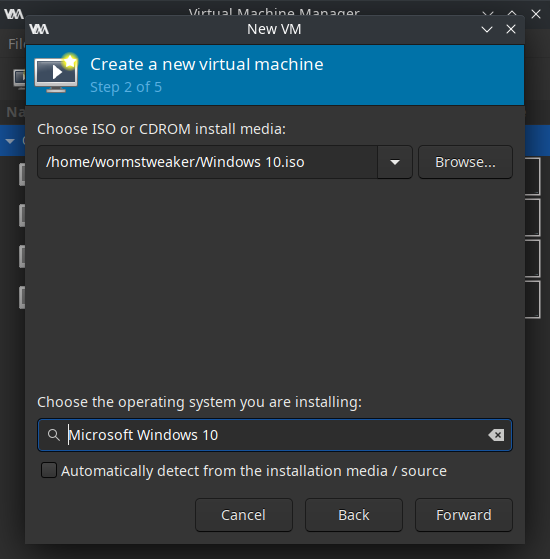
\includegraphics[width=\textwidth]{images/vm-iso-selection.png}
	\end{minipage}
	\begin{minipage}[b]{0.4\textwidth}
		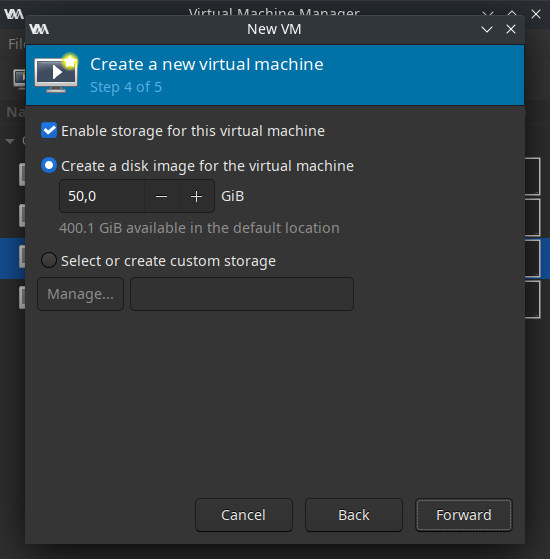
\includegraphics[width=\textwidth]{images/vm-disk-creation.png}
	\end{minipage}
\end{figure}

Vamos a asignarle la memoria RAM \textit{(mi recomendación es asignar, como mínimo, 8GB)} a nuestra máquina virtual. Y en el último paso, vamos a elegir el \textit{customizar nuestra máquina virtual antes de la instalación} (Señalado en la imágen).

\begin{figure}[h]
	\centering
	\begin{minipage}[b]{0.4\textwidth}
		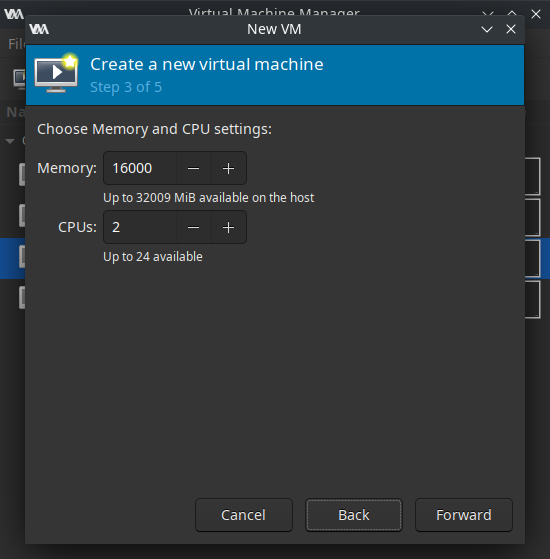
\includegraphics[width=\textwidth]{images/vm-memory-setup.png}
	\end{minipage}
	\begin{minipage}[b]{0.4\textwidth}
		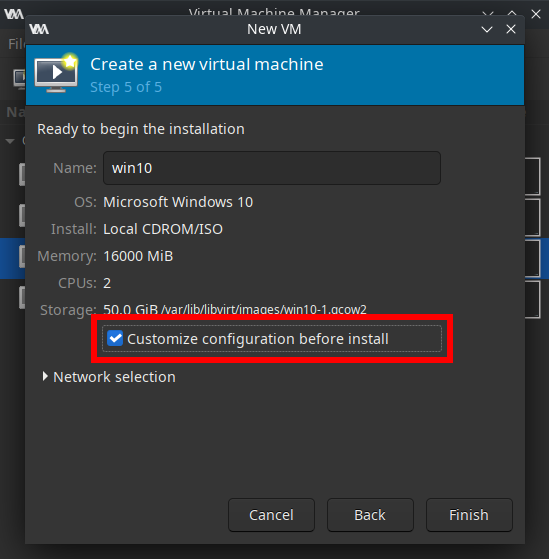
\includegraphics[width=\textwidth]{images/vm-name.png}
	\end{minipage}
\end{figure}

Ahora deberás hacer las siguientes modificaciones:

\begin{itemize}
\setlength\itemsep{-0.3em}
\item Cambiar el chipset a \textit{Q35}
\item Elegir el firmware \path{UEFI: x86_64: /usr/share/edk2/x64/OVMF_CODE.fd}
\item En la pestaña \textit{CPUs} activa el recuadro \textit{Copiar configuración de la CPU del anfitrión}, despliega el menú \textit{Topología} y ajusta la topología de la forma siguiente:
\vspace{-20pt}
\begin{itemize}
	\item 1 \textit{Socket}, Tantos \textit{Centros} comos núcleos tenga tu procesador y tantos \textit{Hilos} como hilos tenga tu procesador por núcleo. Por ejemplo para un procesador con 8 núcleos y 16 hilos, elegiríamos: \textit{1 Socket, 8 Centros, 2 Hilos}. Esto es, si queremos asignar todos los núcleos a nuestra máquina virtual.
\end{itemize}
\item Nos dirigimos a \textit{SATA Disk 1} y cambiamos el bus a VirtIO, de forma que ahora aparezca \textit{VirtIO Disk 1}. Abrimos las opciones avanzadas, y cambiamos el modo de caché a \textit{writeback}.
\item En los ajustes del \textit{NIC} cambiamos el modelo de dispositivo a \textit{virtio}
\item Por último dale a \textit{Añadir hardware} y añade un almacenamiento de tipo de dispositivo CDROM y escribe al lado de \textit{Administrar...} la localización de el ISO con los drivers virtio, por ejemplo: \textit{/home/usuario/Downloads/virtio-win.iso}.
\end{itemize}

\begin{figure}[h!]
	\centering
	\begin{minipage}[b]{0.4965\textwidth}
		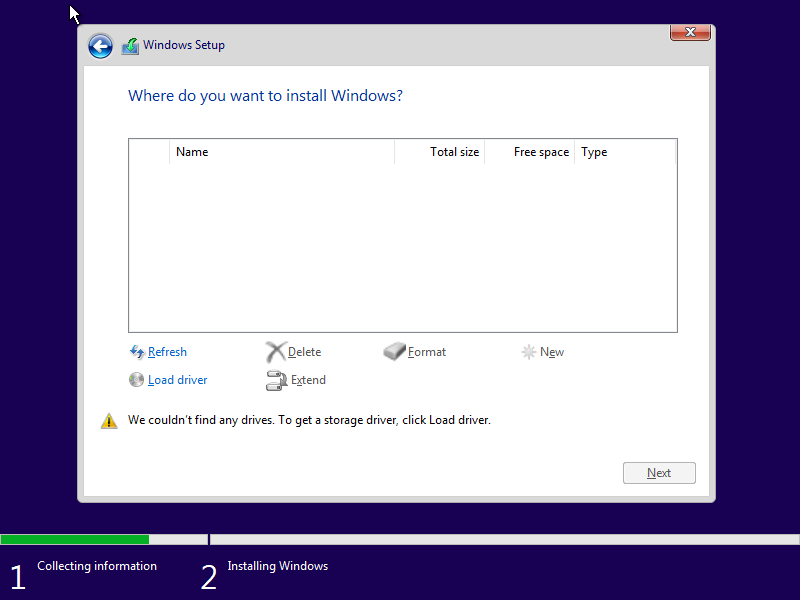
\includegraphics[width=\textwidth]{images/windows-setup-01.png}
	\end{minipage}
	\begin{minipage}[b]{0.4965\textwidth}
		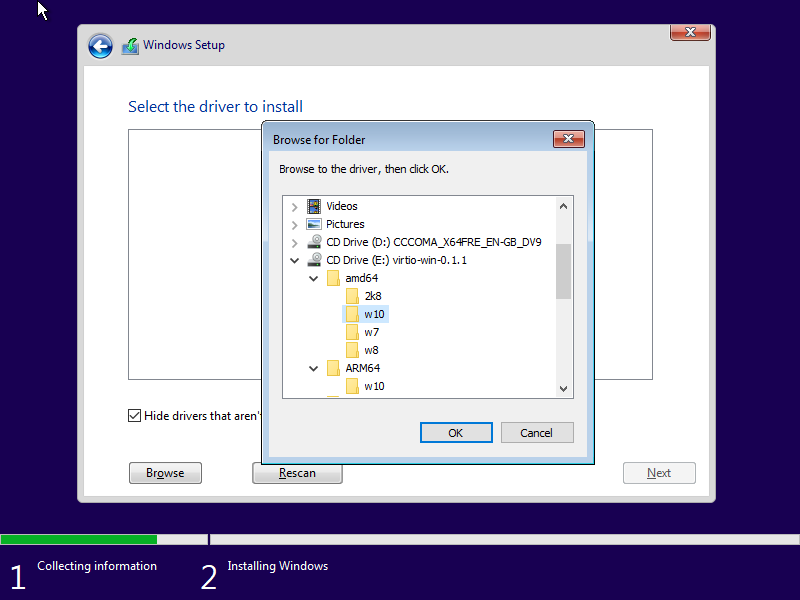
\includegraphics[width=\textwidth]{images/windows-setup-02.png}
	\end{minipage}
\end{figure}

Dale a \textit{Iniciar la instalación} y cuando veas la selección de disco del instalador de windows verás que está vacío. Primero debes darle a \textit{Cargar driver} o \textit{Load driver}, en inglés.

\vspace{5pt}

Selecciona el CD con los drivers virtio y la carpeta que contiene los drivers para Windows 10. Entonces aparecerá tu disco duro virtual y podrás continuar la instalación de Windows. Cuando esta finalize, apaga la máquina virtual.

\begin{figure}[h!]
	\centering
	\begin{minipage}[b]{0.4965\textwidth}
		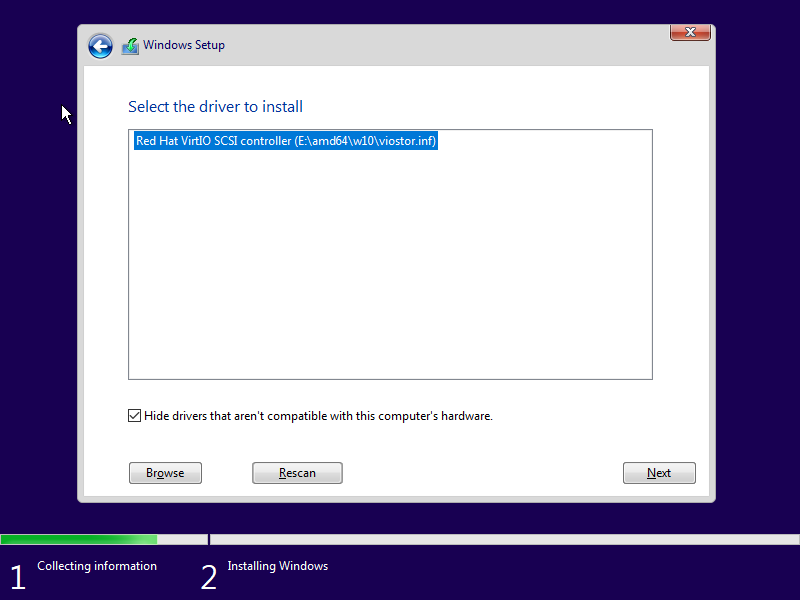
\includegraphics[width=\textwidth]{images/windows-setup-03.png}
	\end{minipage}
	\begin{minipage}[b]{0.4965\textwidth}
		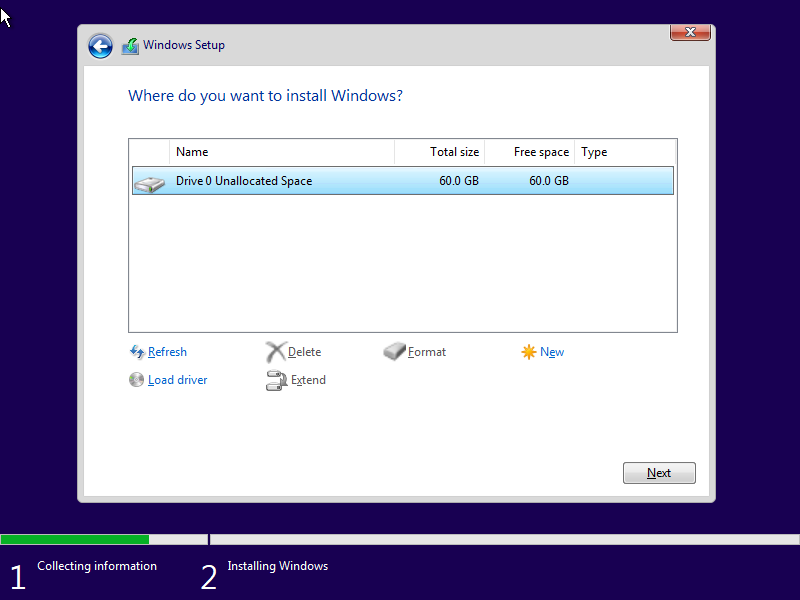
\includegraphics[width=\textwidth]{images/windows-setup-04.png}
	\end{minipage}
\end{figure}

\subsection{Looking Glass en el Host}

Para poder usar nuestra máquina virtual de forma cómoda vamos a configurar \href{https://looking-glass.io/}{Looking Glass}. Una aplicación que nos permite ver la pantalla conectada a nuestra gráfica a través de una ventana y poder controlar nuestra máquina virtual sin necesidad de conectar un teclado y ratón sólo para nuestra máquina virtual. El único problema es que para usar looking glass sin necesidad de dos monitores, necesitamos comprar un \href{https://www.amazon.com/s?k=display+dummy}{display dummy}. Por lo menos, su precio suele rondar los 5-7€.

\vspace{5pt}

Looking Glass nos muestra una imagen de lo que esta haciendo nuestra gráfica con una latencia muy baja, suficiente para poder jugar a juegos o editar vídeo \textit{(y otros usos posibles)} sin problema en nuestra máquina virtual. Logra esto mandando la información a través de un archivo compartido entre máquina virtual y host.

Primero necesitamos configurar \href{dsada}{tmpfilesd} para que cada vez que iniciamos el sistema, cree el archivo que compartirán máquina virtual y host para enviarse información. Tenemos que ejecutar el siguiente comando \textit{(sustituyendo usuario por el nombre de tu usuario)}:

\begin{verbatim}
echo "f /dev/shm/looking-glass 0660 usuario kvm -" | \
doas tee -a /etc/tmpfiles.d/looking-glass.conf
\end{verbatim}

Tenemos que instalar el servicio que se encarga de crear estos archivos con:

\begin{verbatim}
doas pacman -Sy --noconfirm etmpfiles
\end{verbatim}

\subsection{Añadir Gráfica y Looking Glass en el Guest}

Ahora ya tenemos casi todo listo, queda instalar los drivers de vídeo e instalar Looking Glass en nuestra máquina virtual \textit{(a la hora de la instalación debió de haberse instalado ya en nuestro linux)}.

\vspace{5pt}

Primero tenemos que añadir nuestra tarjeta gráfica a nuestra máquina virtual. Para ello tenemos que ir a los ajustes de nuestra máquina virtual y en \textit{``Añadir Dispositivo"}, busca la pestaña para añadir dispositivos PCI y añade tu gráfica.

\vspace{5pt}

Después debemos de configurar el servidor Spice para que use el puerto 6000 en vez de asignar un puerto automáticamente

\begin{figure}[h!]
	\centering
	\begin{minipage}[b]{0.4965\textwidth}
		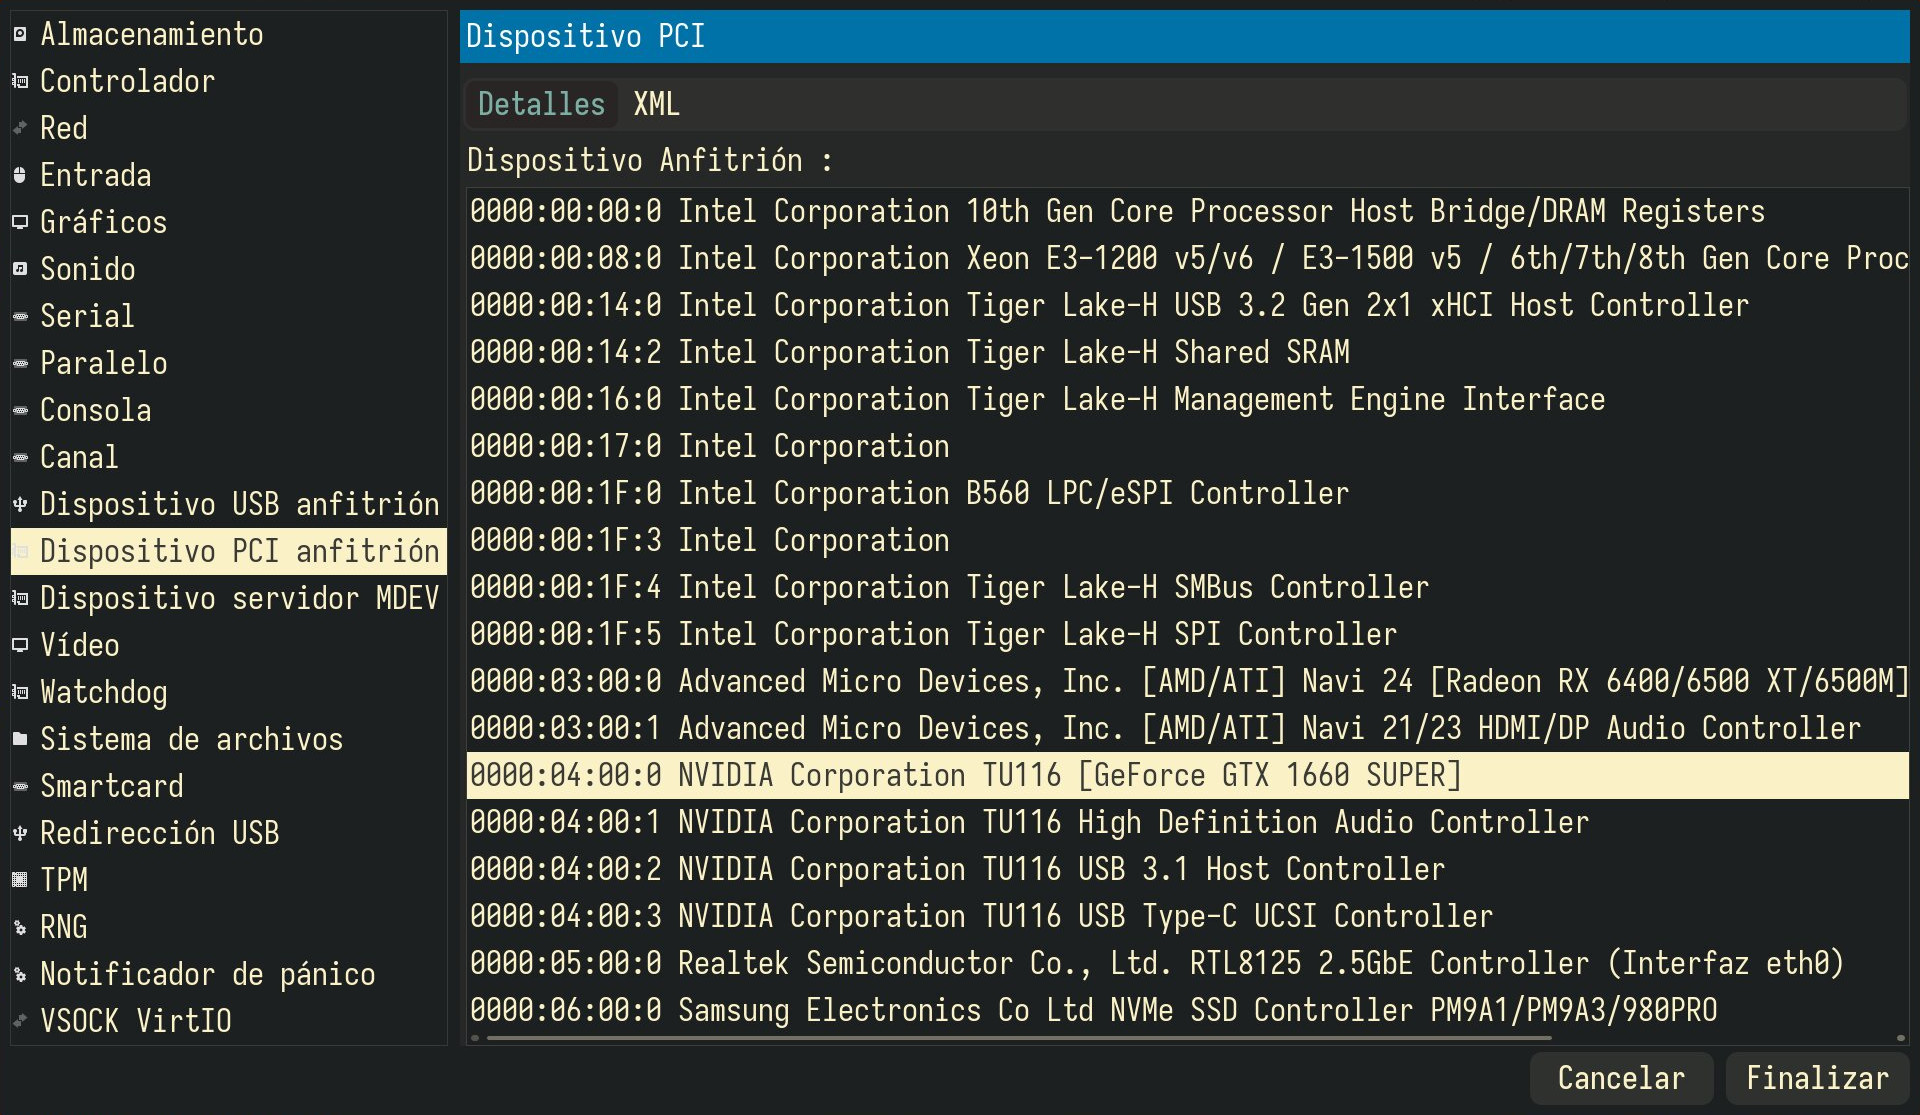
\includegraphics[height=0.6\textwidth,width=\textwidth]{images/card-add.jpg}
	\end{minipage}
	\begin{minipage}[b]{0.4965\textwidth}
		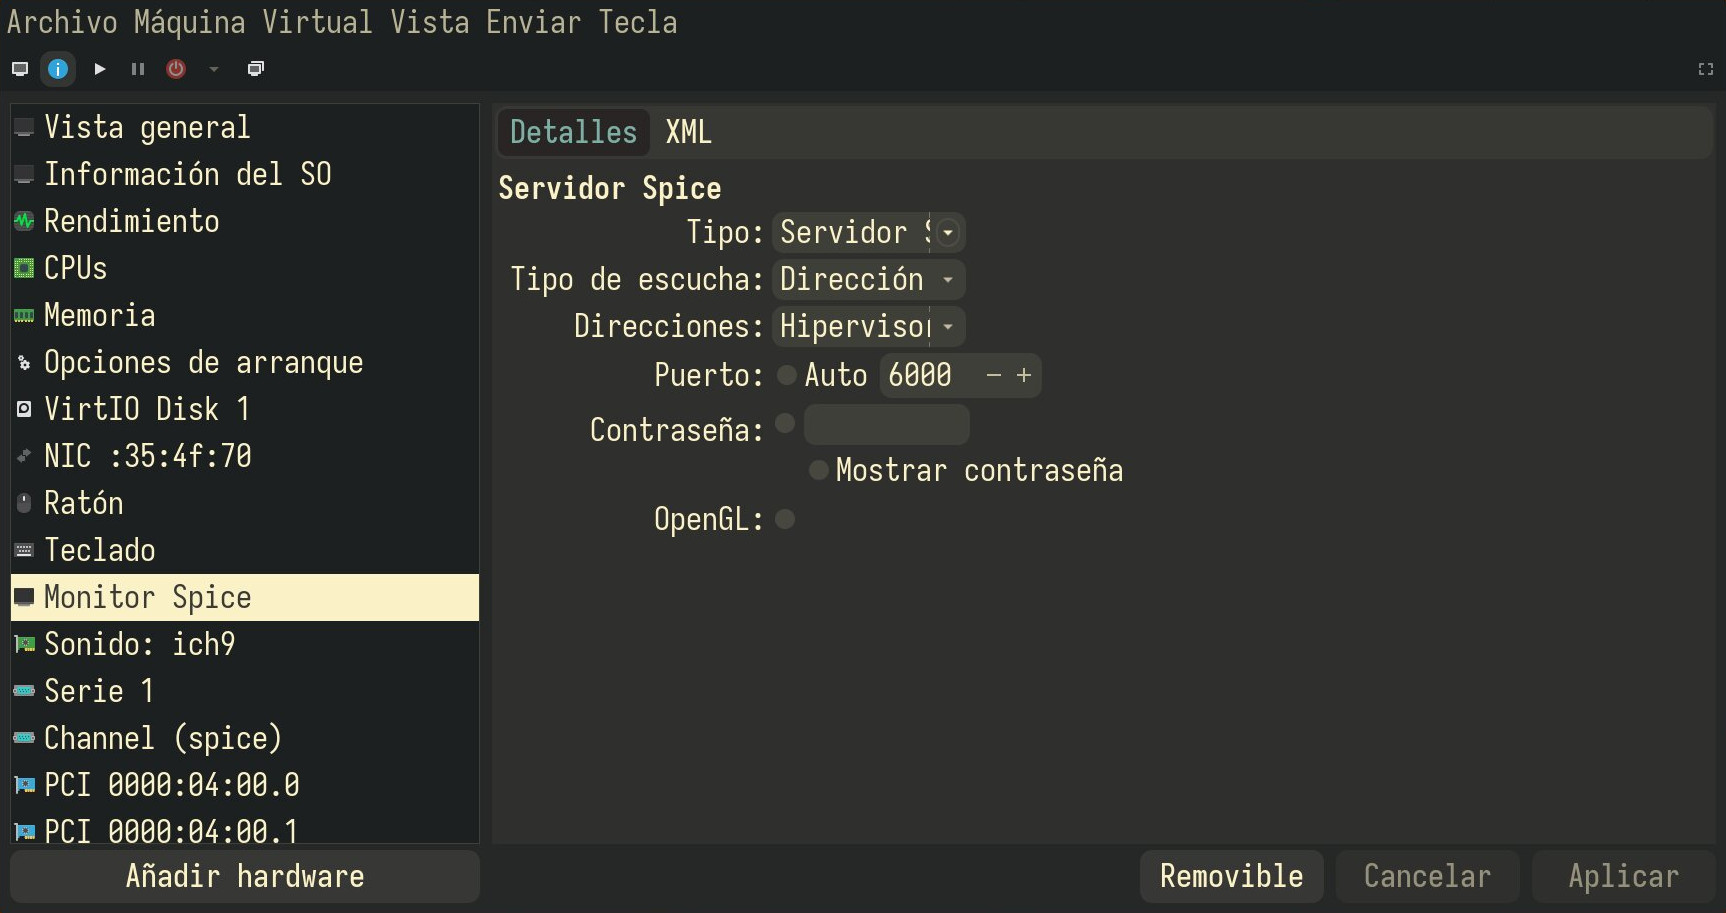
\includegraphics[height=0.6\textwidth,width=\textwidth]{images/spice-conf.jpg}
	\end{minipage}
\end{figure}

Ahora tenemos que activar la edición de XML en Virt-Manager (Editar $\to$ Preferencias) y editar el código XML de nuestra máquina virtual. Añadiremos estas lineas de código al final para que el archivo acabe viéndose así:

\begin{figure}[h!]
	\centering
	\begin{minipage}[b]{0.3285\textwidth}
		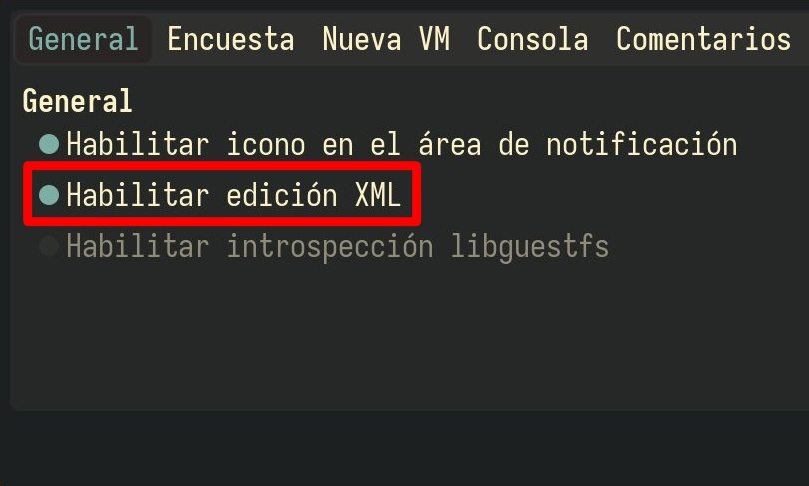
\includegraphics[height=0.6\textwidth,width=\textwidth]{images/xml-enable.jpg}
	\end{minipage}
	\begin{minipage}[b]{0.3285\textwidth}
		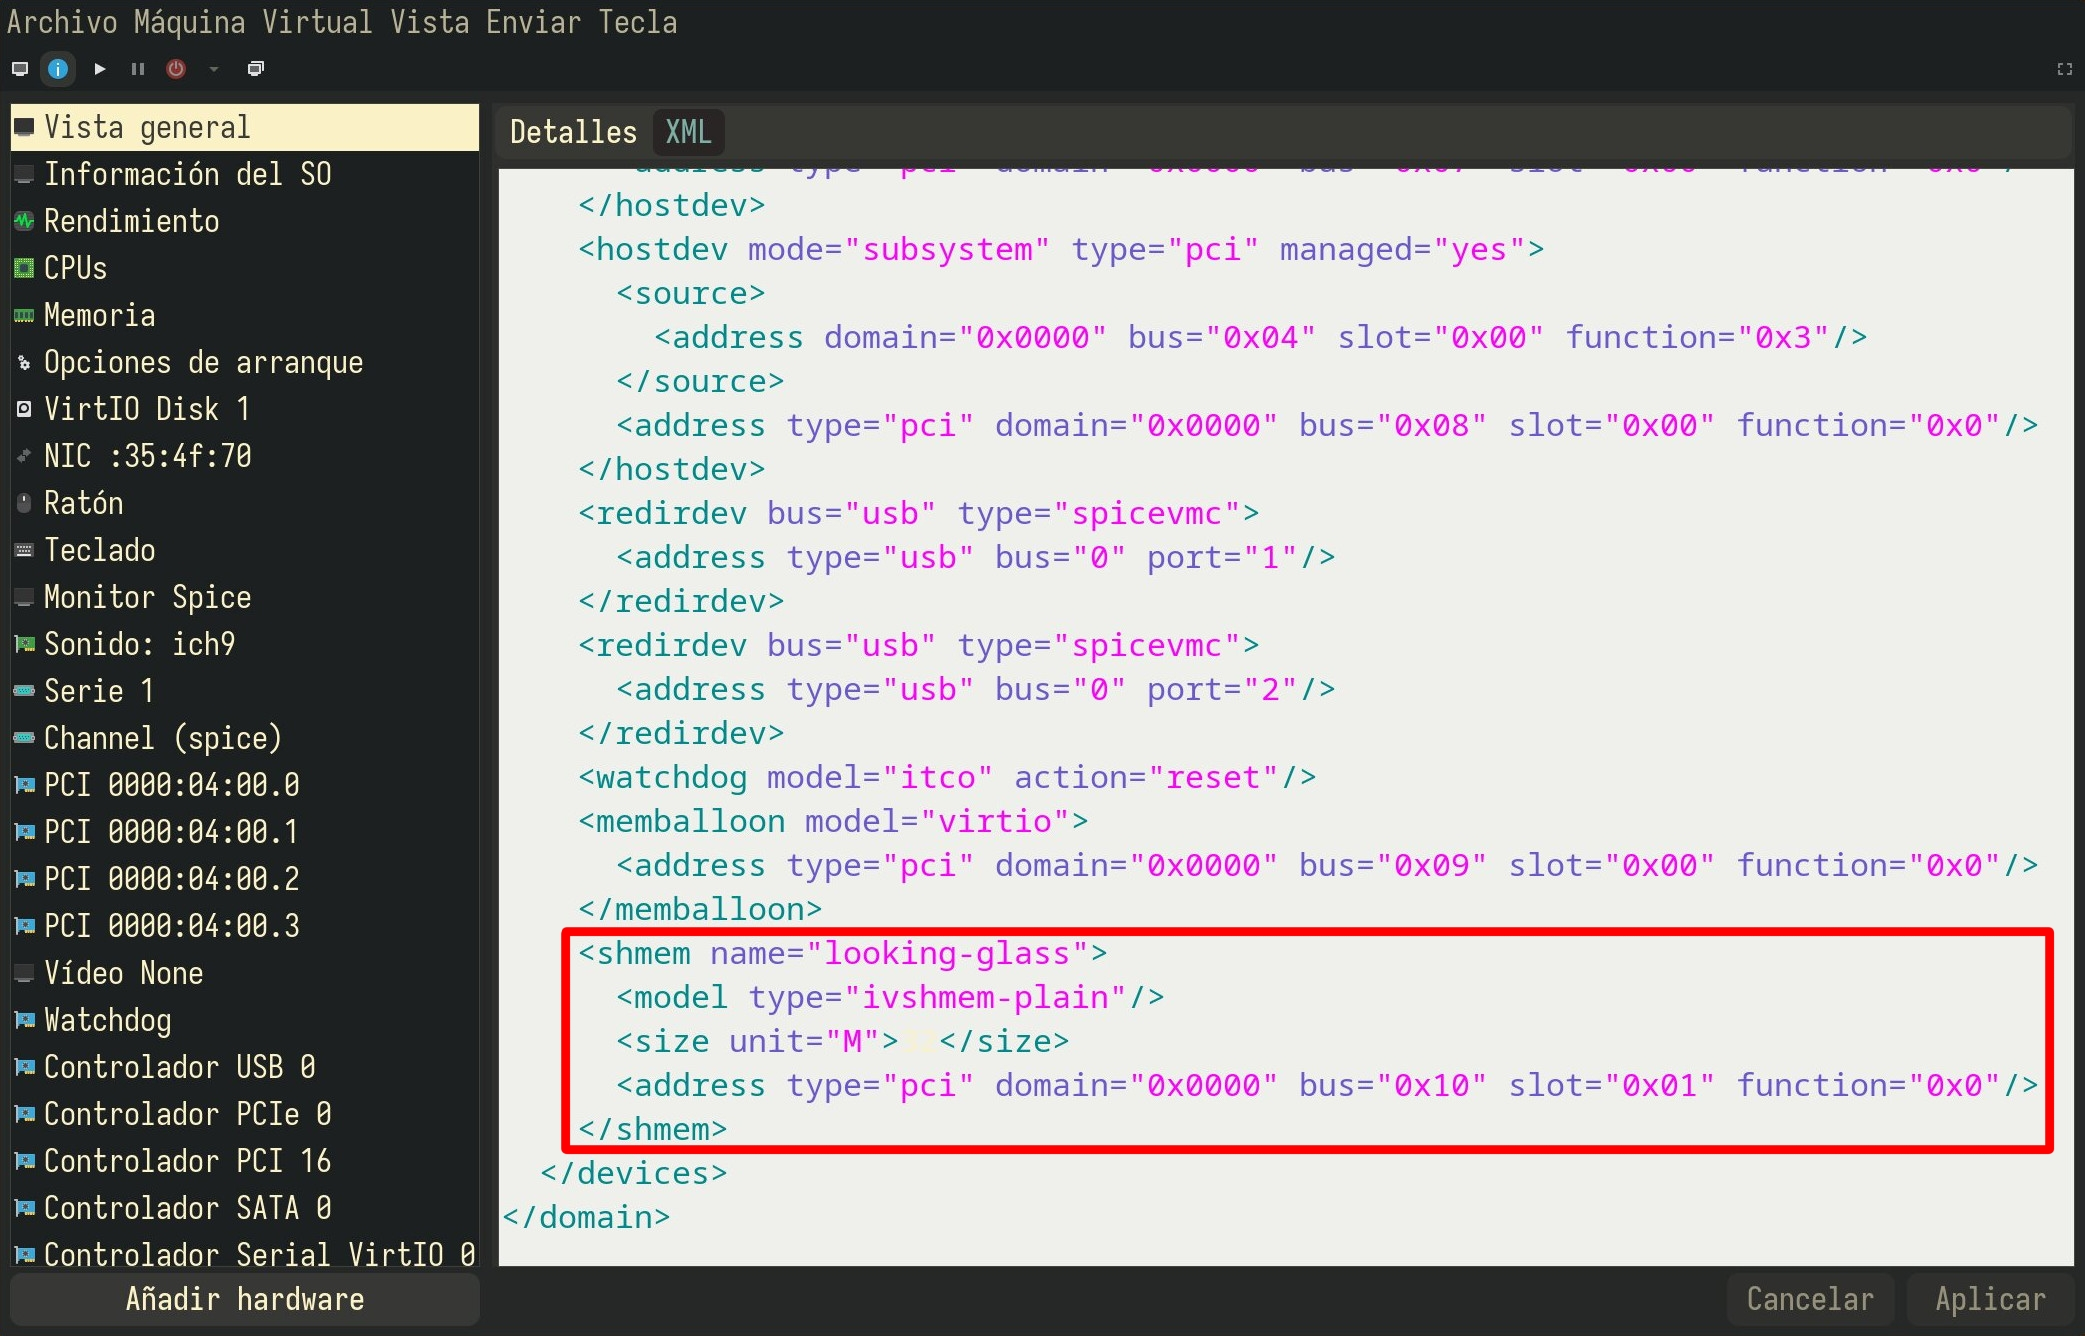
\includegraphics[height=0.6\textwidth,width=\textwidth]{images/xml-edit.jpg}
	\end{minipage}
	\begin{minipage}[b]{0.3285\textwidth}
		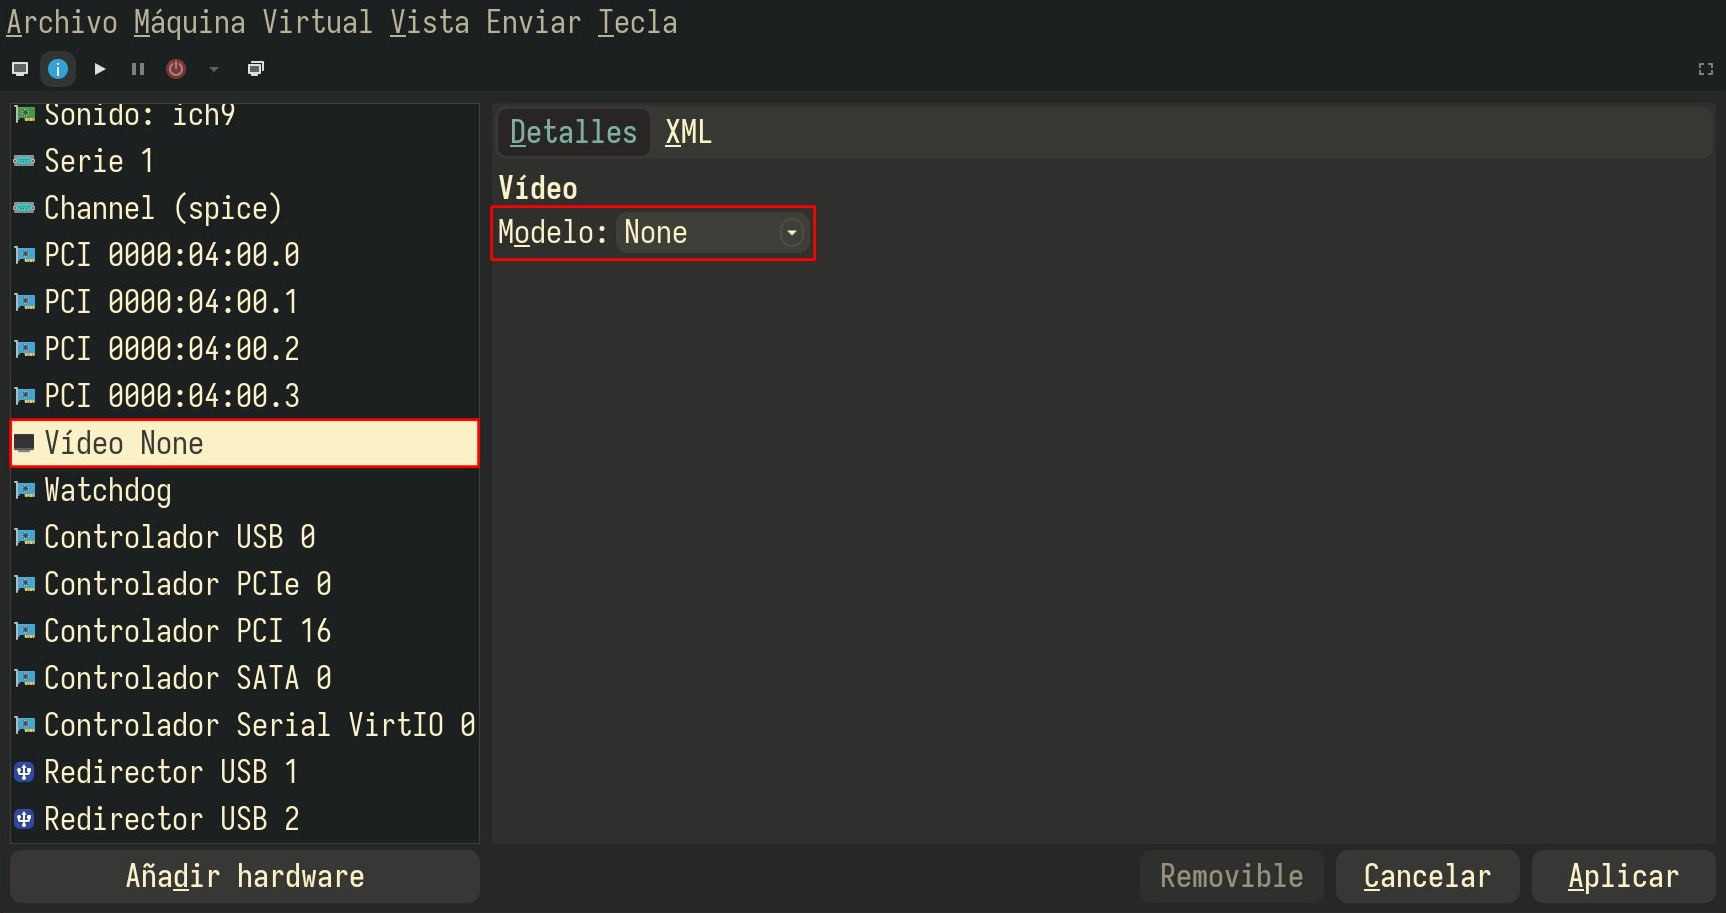
\includegraphics[height=0.6\textwidth,width=\textwidth]{images/video-none.jpg}
	\end{minipage}
\end{figure}

Iniciamos nuestra máquina virtual e instalamos nuestros drivers de \href{https://www.nvidia.es/Download/index.aspx?lang=es}{NVIDIA} o \href{https://www.amd.com/es/support}{AMD} y \href{https://looking-glass.io/downloads}{Looking Glass Host}.

\vspace{5pt}

Finalmente cambiamos el driver virtual de video de \textit{QXL} a \textit{None} y borramos el dispositivo de tableta táctil. La próxima vez que iniciemos la máquina virtual solo tenemos que iniciarla en Virt-Manager e ínteractuaremos con nuestra máquina virtual abriendo Looking Glass \textit{(Podemos abrirlo seleccionando ``Looking Glass`` en el menú que aparece cuando hacemos clic derecho en alguna parte vacía del Escritorio)}.

\clearpage

\noindent Para que esto funcione debemos reiniciar nuestro ordenador o ejecutar el comando.

\begin{verbatim}
doas install -g kvm -o $(whoami) -m 0660 /dev/null /dev/shm/looking-glass
\end{verbatim}

\begin{mybox}{Nota}

Para más información sobre como configurar un VFIO passthought puede consultar:

\vspace{-7.5pt}

\begin{itemize}
\setlength\itemsep{-0.3em}
\item \href{https://qqq.ninja/blog/post/vfio-on-arch/}
{https://qqq.ninja/blog/post/vfio-on-arch/}
\item \href{https://gitlab.com/risingprismtv/single-gpu-passthrough/-/wikis/home}
{https://gitlab.com/risingprismtv/single-gpu-passthrough/-/wikis/home}
\item \href{https://wiki.archlinux.org/title/PCI\_passthrough\_via\_OVMF}
{https://wiki.archlinux.org/title/PCI\_passthrough\_via\_OVMF}
\end{itemize}
\end{mybox}

\section{VirtioFS}

Podemos usar virtiofs para compartir directorios del host con nuestra máquina virtual. Para ello, necesitamos añadir los directorios deseados desde Virt-Manager, seleccionando: Añadir hardware, Sistema de archivos, eligiendo la Ruta de origen (la carpeta que queremos compartir) y la Ruta objetivo (el nombre con el que aparecerá en nuestra máquina invitada).

\vspace{5pt}

También necesitamos instalar los controladores de VirtIO en el host. Si todavía tenemos montado el disco que contiene estos controladores, encontraremos en el CD un instalador (virtio-win-gt-x64.msi) para los controladores, así como otro instalador \emph{opcional} para añadir la integración con el host (virtio-win-guest-tools.exe), que permite funciones como compartir el portapapeles, entre otras.

\vspace{5pt}

Después de instalar los controladores, debemos instalar \href{https://github.com/winfsp/winfsp}{WinFSP} para poder montar sistemas de archivos VirtioFS.

\vspace{5pt}

Una vez que tenemos todo instalado, podemos crear un script `.bat` que monte nuestras carpetas en la máquina invitada. Por ejemplo, si tenemos dos carpetas cuyas rutas objetivo son ``documentos'' y ``videos'', y queremos montarlas en ``Y:'' y ``Z:'', respectivamente, podemos crear un script para montar ambas de la siguiente manera:

\vspace{5pt}

\begin{lstlisting}[basicstyle=\scriptsize\ttfamily]
"C:\Program Files (x86)\WinFsp\bin\launchctl-x64.exe" start virtiofs documentos documentos Y:
"C:\Program Files (x86)\WinFsp\bin\launchctl-x64.exe" start virtiofs videos videos Z:
\end{lstlisting}

\section{Conexión bridge y RDP}

Adicionalmente, podemos configurar nuestra máquina virtual para, a efectos prácticos, comportarse como un ordenador distinto en la red. En vez de usar un NAT y que nuestro host se encargue del re-direccionamiento al guest, podemos usar una conexión puente y hacer que nuestro router reconozca nuestra máquina virtual como un dipositivo distinto y le asigne su propia IP. Esto es útil para abrir servicios desde nuestro guest y poder alcanzarlos desde el exterior de nuestra red privada.

\subsection{Creación de nuestra red puente}

Para crear nuestra conexión de puente, utilizaremos \emph{NetworkManager}. Podemos configurar nuestras conexiones a través de la terminal usando \texttt{nmtui}. Al ejecutar \texttt{nmtui}, seleccionaremos \emph{Modificar una conexión} y luego \emph{<Añadir>}. En el tipo de red, escogeremos \emph{Puente}.

Una vez que seleccionemos el dispositivo tipo \emph{Puente}, aparecerán las distintas opciones de configuración de nuestra red. Procederemos a configurar el dispositivo que queremos puentear; para ello, en la sección \emph{Puente, ports}, seleccionamos \emph{<Añadir>} y elegimos \emph{<Ethernet>} (Nota: esto solo funciona correctamente para dispositivos conectados mediante Ethernet; no es posible utilizar conexiones puenteadas a través de Wi-Fi). Luego, seleccionamos \emph{<Crear>} y finalmente \emph{<Aceptar>}. Por último, confirmaremos los cambios para agregar nuestra conexión de puente.

Finalmente, debemos eliminar la conexión Ethernet de la lista de conexiones en \emph{NetworkManager} (no te preocupes, tu host seguirá teniendo acceso a internet; tanto la máquina anfitriona como la máquina invitada usarán la conexión de puente para acceder a internet). Para ello, en \texttt{nmtui} seleccionamos \emph{Modificar una conexión} y eliminamos la conexión correspondiente.

\subsection{Invitado con conexión puenteada}

Ahora tenemos que decirle a virt-manager que queremos usar nuestra conexión puenteada para la máquina virtual, podemos incluso borrar la red NAT \emph{`default"} si no tenemos ninguna otra máquina virtual que queramos conectar a internet.

Para usar la conexión puenteada en nuestra máquina virtual; en las propiedades de nuestra máquina virtual, dentro de la configuración del \textbf{NIC} vamos a elegir en la \emph{`Fuente de red"} nuestra conexión puenteada.

Adicionalmente, podemos ajustar la dirección MAC y establecer una IP estática asociada a esa dirección MAC en nuestro router. Lo cual facilitará confiurar servicios y acceder a nuestra máquina invitada desde la red.

\subsection{Configurar Escritorio remoto}

Ahora podemos configurar nuestra máquina invitada para acceder remotamente a ella mediante RDP, para ello en Windows \emph{(Sólo si tenemos Windows 10/11 Pro)} en Ajustes/Escritorio Remoto, activaremos el escritorio remoto.

Es recomendable configurar el firewall de nuestro guest para permitir las conexiones entrantes de RDP y ICMP, para ello ejecutaremos estos comandos en la Consola de Comandos como Administrador:

\begin{lstlisting}[basicstyle=\tiny\ttfamily]
netsh advfirewall firewall add rule name="Allow ICMPv4-In" protocol=icmpv4:any,any dir=in action=allow
netsh advfirewall firewall add rule name="Allow ICMPv6-In" protocol=icmpv6:any,any dir=in action=allow
netsh advfirewall firewall add rule name="Allow RDP" protocol=TCP dir=in localport=3389 action=allow
\end{lstlisting}

Podemos conectarnos ya a nuestra máquina usando freerdp con el comando

\begin{lstlisting}[basicstyle=\small\ttfamily]
xfreerdp3 /u:USUARIO /p:'CONTRASEÑA' /v:IP /auth-pkg-list:'!kerberos' \
	/sound:sys:alsa /size:1920x1080 /smart-sizing:1920x1080 +clipboard
\end{lstlisting}

O puedes usar el script \texttt{rdp-connect}

\section{SSH}

Si queremos conectarnos a un equipo remoto a través de internet debemos configurar \href{https://es.wikipedia.org/wiki/OpenSSH}{OpenSSH}. Por defecto incluyo un script que configura SSH de forma muy básica, configurando SSH para poder acceder a tu equipo remoto con una contraseña. Para activar SSH simplemente ejecuta:

\begin{verbatim}
ssh-configure
\end{verbatim}

Mi recomendación es no conformarse con esta configuración básica. Desactiva el login con el usuario root, desactiva el login por contraseña y usa claves públicas para conectarte. Si no sabes de lo que estoy hablando, es mejor que no uses SSH y no te expongas a abrir la puerta a tu ordenador al internet, aunque sea con candado.

\subsection{VNC através de SSH}

Podemos usar SSH para acceder a nuestro entorno gráfico de forma remota y usar nuestro ordenador sin estar necesariamente delante de el físicamente. Por defecto dwm inicia un servidor \href{https://en.wikipedia.org/wiki/Virtual_Network_Computing}{VNC} para que puedas conectarte remotamente a una interfaz gráfica. Para poder hacer uso del servidor VNC tienes que usar \href{https://en.wikipedia.org/wiki/Tunneling_protocol}{tunneling}. Para conectarte y poder usar VNC, ejecuta:

\begin{verbatim}
ssh usuario@255.255.255.255 -L 5900:localhost:5900
\end{verbatim}

Sustituye \textit{usuario} por el usuario de tu máquina, y \textit{255.255.255.255} por la dirección IP de tu máquina. Para conectarte al equipo remotamente debes tener instalado algún cliente VNC, mi recomendación es \href{https://github.com/FreeRDP/Remmina}{remmina}.

\section{Firewall}

Instalar y configurar un firewall no es posible dentro de un chroot. Por eso configurar el firewall debe hacerse una vez reiniciemos y hallamos arrancado nuestro sistema operativo. Para instalar el firewall ejecuta:

\begin{verbatim}
doas sh -c 'pacman -Sy ufw-openrc; rc-update add ufw default; ufw enable'
\end{verbatim}

Ahora, la próxima vez que inicies tu equipo tendras un firewall ya instalado. Para configurarlo puedes ejecutar los siguientes comandos, que establecen unas reglas de filtrado de paquetes bastante permisivas.

\begin{verbatim}
doas ufw limit 22/tcp; doas ufw allow 80/tcp
doas ufw allow 443/tcp; doas ufw allow syncthing
doas ufw default deny incoming; doas ufw default allow outgoing
\end{verbatim}

\begin{mybox}{Nota}
Si ejecutaste \textit{ssh-configure} el firewall ya se configuró automaticamente
\end{mybox}

\section{Syncthing}

\href{https://github.com/syncthing/syncthing}{Syncthing} es un software para sincronizar archivos entre dispositivos, es lo que uso para poder trabajar en todos mis equipos sin necesidad de estar intercambiando pen-drives como un troglodita.

Viene instalado por defecto y se ejecuta cuando inicias tu ordenador. Para configurarlo tiene una \href{http://localhost:8384/}{interfaz gráfica} a la que puedes acceder desde tu navegador.

\begin{mybox}{Información}
Aquí puedes encontrar documentación sobre como usar syncthing: \href{https://docs.syncthing.net/}{https://docs.syncthing.net/}
\end{mybox}

\section{Monitores de altas tasas de refresco}

Por defecto dwm actualiza el movimiento de las ventanas a 60 FPS. Si tienes un monitor de mas de 60 Hz esto puede hacer la experiencia de usar dwm insatisfactoria. Para cambiar este comportamiento, debes editar el archivo \textit{dwm.c}. En el encontrarás varias funciones con esta misma linea de código:

\begin{verbatim}
if ((ev.xmotion.time - lasttime) <= (1000 / 60))
\end{verbatim}

Deberás cambiar el valor \textit{60} por la tasa de refresco de tu monitor en cada aparición de esta linea. Por ejemplo, para un monitor de \textit{144 Hz}, la líneas a cambiar deberían verse así: \path{if ((ev.xmotion.time - lasttime) <= (1000 / 144))}

\section{Firefox}

\subsection{Cambiar buscador por defecto}

\vspace{-15pt}

\begin{figure}[h!]
	\fcapside[\FBwidth]{\caption*{Pese a usar \href{https://github.com/arkenfox/user.js}{arkenfox} para mejorar algunos ajustes relacionados con la privacidad, el buscador por defecto sigue siendo Google. Es recomendable cambiarlo por alguno como \href{https://search.brave.com/}{Brave Search} o \href{https://duckduckgo.com/}{DuckDuckGo}.}}
{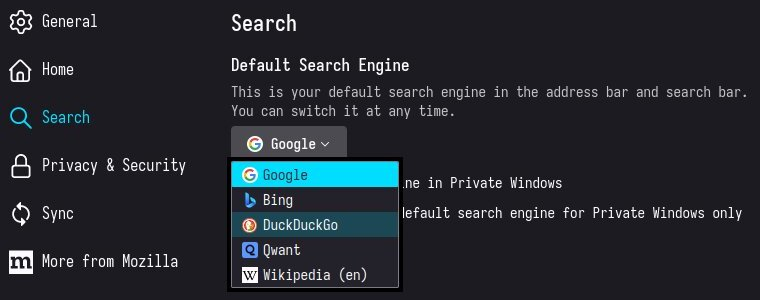
\includegraphics[width=0.5\textwidth,height=0.175\textwidth]{images/search-engine.jpg}}
\end{figure}%

\vspace{-20pt}

\subsection{Violentmonkey}

Violentmonkey es una extensión para cargar pequeños scripts de javascript justop después de cargar la página web, para automatizar ciertas tareas o añadir funcionalidades. Si vas a los ajustes de la extensión, verás que hay una pestaña donde puedes importar tus ajustes. Podemos importar nuestros ajustes que están en el archivo:

\begin{figure}[h!]
	\captionsetup{labelformat=empty}
	\centering
	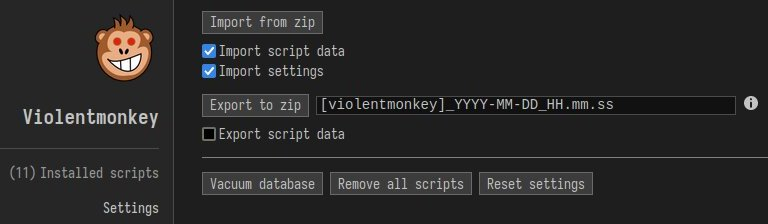
\includegraphics[width=0.6\textwidth]{images/violentmonkey.jpg}
	\cprotect\caption{\verb|~/.dotfiles/assets/violentmonkey.zip|}
\end{figure}

\vspace{-20pt}

\subsection{Añadir buscadores útiles}

Aquí tienes una lista de buscadores útiles, para añadirlos a tu buscador simplemente accede a cada página haciendo doble clic, y cuando estés en ella haz clic derecho en la barra de navegación y selecciona \textit{Añadir "Buscador"}.

\begin{multicols}{5}
\scriptsize
\begin{itemize}
\setlength\itemindent{-0.75em}
\setlength\itemsep{-0.35em}
\item \href{https://wiki.archlinux.org/}{Arch Wiki}
\item \href{https://wiki.gentoo.org/wiki/Main_Page}{Gentoo Wiki}
\item \href{https://wiki.alpinelinux.org/wiki/Main_Page}{Alpine Wiki}
\item \href{https://www.youtube.com/}{YouTube}
\item \href{https://nyc1.pi.ggtyler.dev/trending}{Piped}
\item \href{https://iv.ggtyler.dev/feed/popular}{Invidious}
\item \href{https://github.com/}{GitHub}
\item \href{https://yandex.com/}{Yandex}
\item \href{https://nyaa.si/}{Nyaa}
\item \href{https://stackoverflow.com/}{Stack Overflow}
\end{itemize}
\end{multicols}

Las Wikis de Gentoo y Alpine nos resultarán de utilidad, pues ambas distribuciones utilizan OpenRC en vez de SystemD. De hecho, si no encuentras un script de OpenRC para algún servicio en los repositorios de Artix, puedes copiar el script que utilizan Alpine o Gentoo.

\section{Miscelánea}

\subsection*{Configuraciones locales}

Nuestra configuración de \texttt{zsh} tiene varios \emph{alias} configurados en:

\begin{center}
\path{~/.config/zsh/aliasrc}
\end{center}

Si deseamos añadir alias de forma no global, sin tener que añadir archivos al repositorio y de manera exclusiva para nuestro equipo, podemos crear un archivo con más funciones y abreviaciones en:

\begin{center}
\path{~/.config/useralias}
\end{center}

\subsection*{Aviso de Uso}

Este proyecto es para uso personal. Se comparte con la intención de que pueda ser útil para otros, pero se proporciona tal cual, sin ninguna garantía. No se asume responsabilidad por ninguna pérdida de datos o problemas que puedan surgir del uso de este proyecto.

\vspace{5pt}

No obstante, se aceptan propuestas de mejora razonables. Si alguien desea contribuir a hacer este setup más extensible y robusto, puede realizar un merge request sin inconveniente.

\end{document}
